\documentclass[11pt]{scrartcl}

\usepackage[top=1in, bottom=2cm, left=1in, right=1in]{geometry}
\usepackage{graphicx}
\usepackage{amsmath}

\begin{document}

\title{HW5 STAT5376}
\subtitle{Dynamic programming with SRSF}
\author{Li Sun}
\date{\today}
\maketitle

\noindent
PART I: Smooth function registration\\
To demonstrate the dynamic programming with SRSF, I simulated several pairs of functions and try to register them.\\
1.First to register two identical function.\\
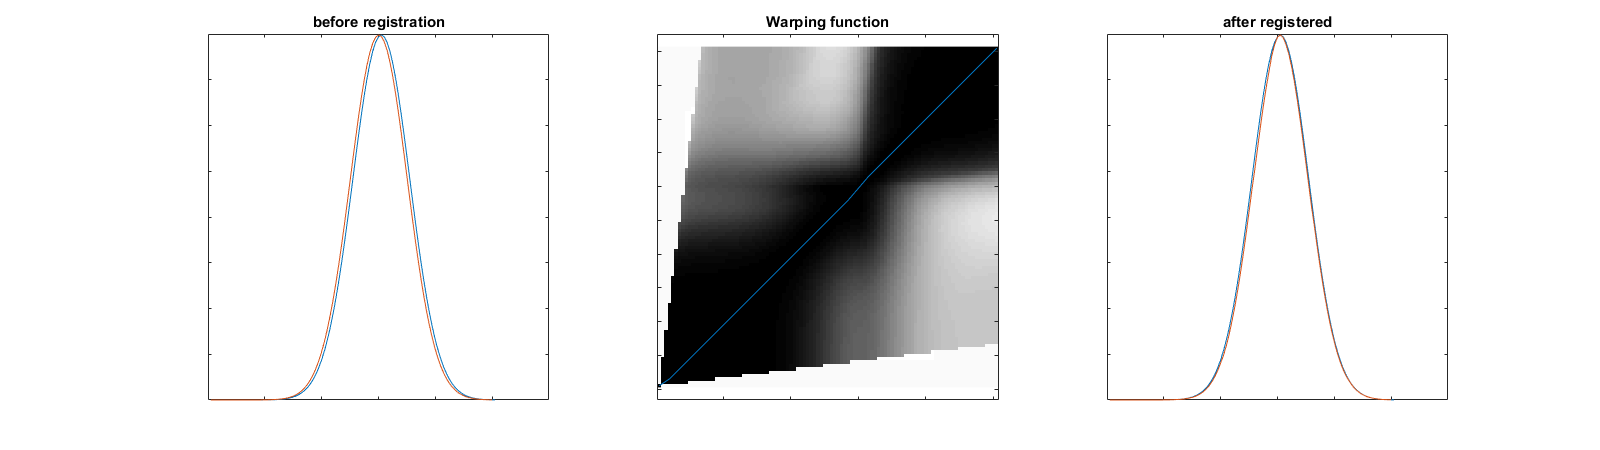
\includegraphics[scale=0.4]{hw51.png}\\
da=0\\
dp=0\\
2.Register 2 functions with different locations but exact same shapes\\
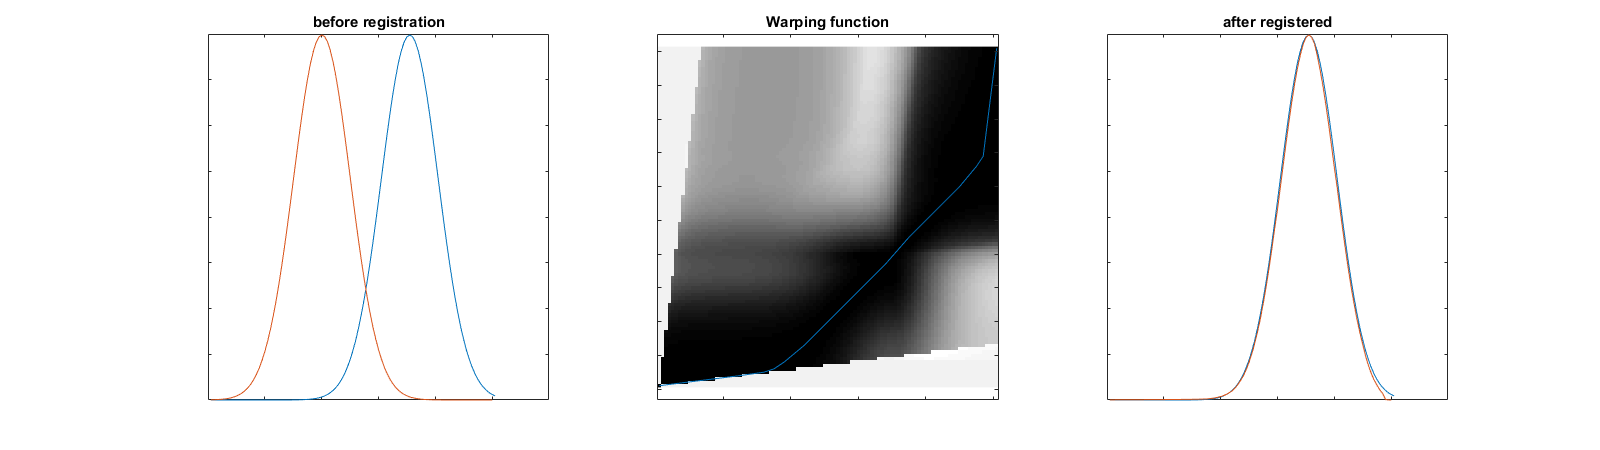
\includegraphics[scale=0.4]{hw52.png}\\
da=0.0466\\
dp=0.8591\\
3.Functions with different variation but same location.\\
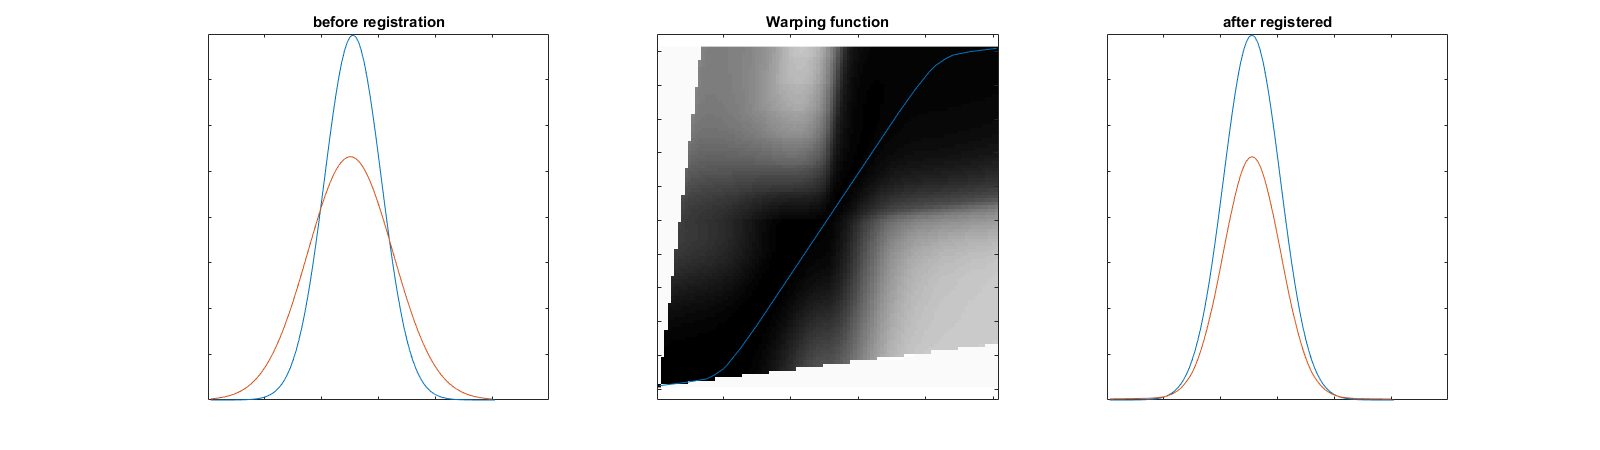
\includegraphics[scale=0.4]{hw53.png}\\
da=0.2688\\
dp=1.2325\\
4.Functions with different center and different variations.\\
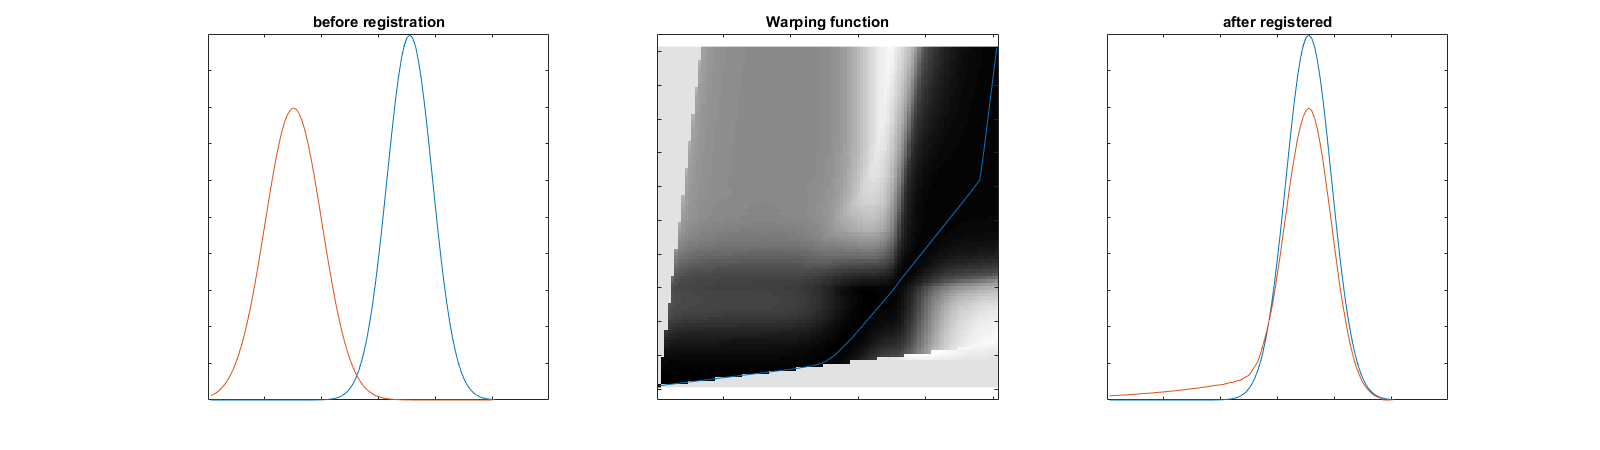
\includegraphics[scale=0.4]{hw54.png}\\
da=0.3638\\
dp=1.0277\\
5.Let's try warp bi-peak function.\\
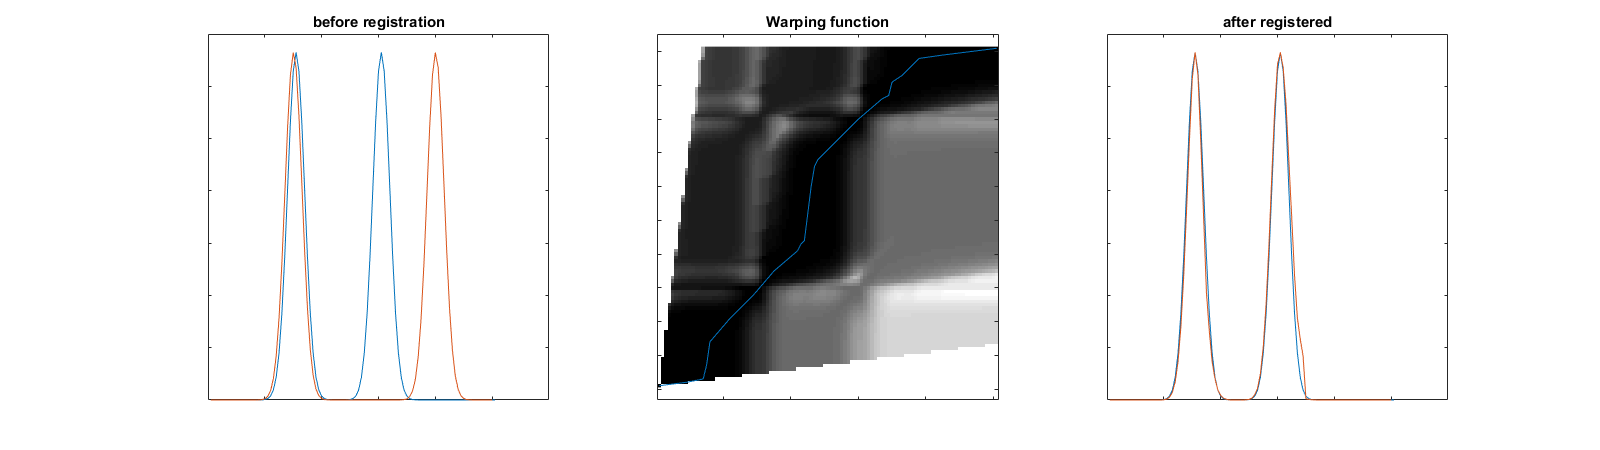
\includegraphics[scale=0.4]{hw55.png}\\
da=0.0014\\
dp=0.3911\\
6.If warp g to f, can we observe inverted warping function?\\
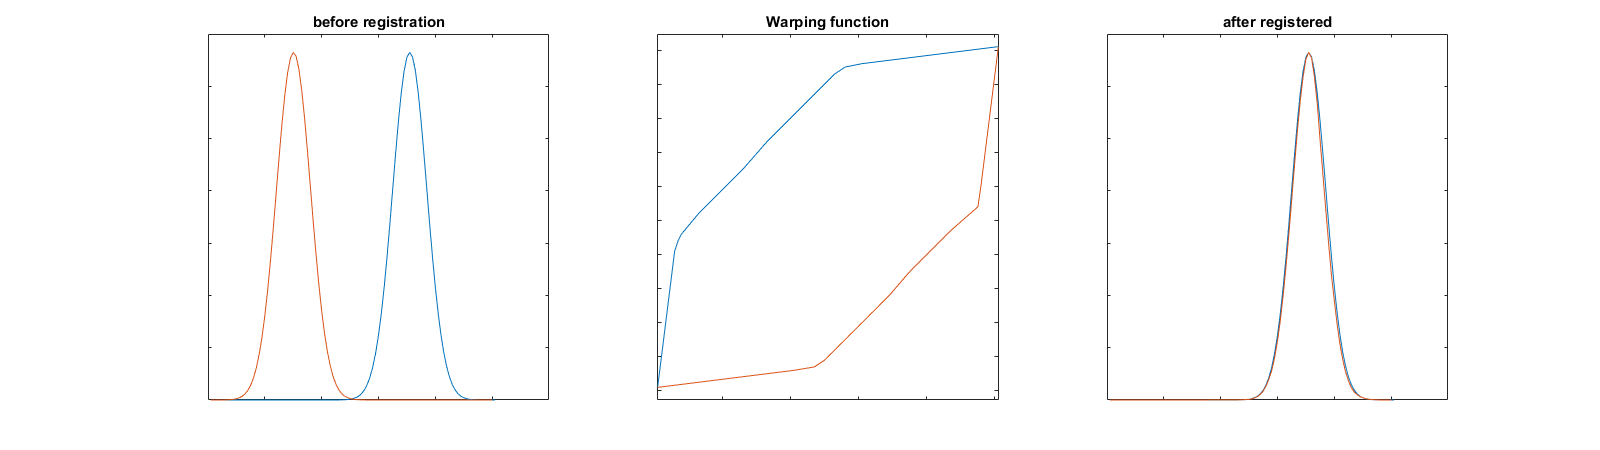
\includegraphics[scale=0.4]{hw56.png}\\
Above all, the algorithm searches 43 points as neighbors with 43 different slopes. It calculate fast and works well under most situations.Indeed, if we change the order of 2 functions to be warped, the warping function is inverse to each other.\\
However, I do observed some distortion when I tried to register a curve with larger magnitude to another curve with lower magnitude. The magnitude is well reserved which is an improvement comparing to L2-norm registration.\\

\bigskip

PART II: smooth and register growth data.\\
Data from R package fda as in following figure:\\
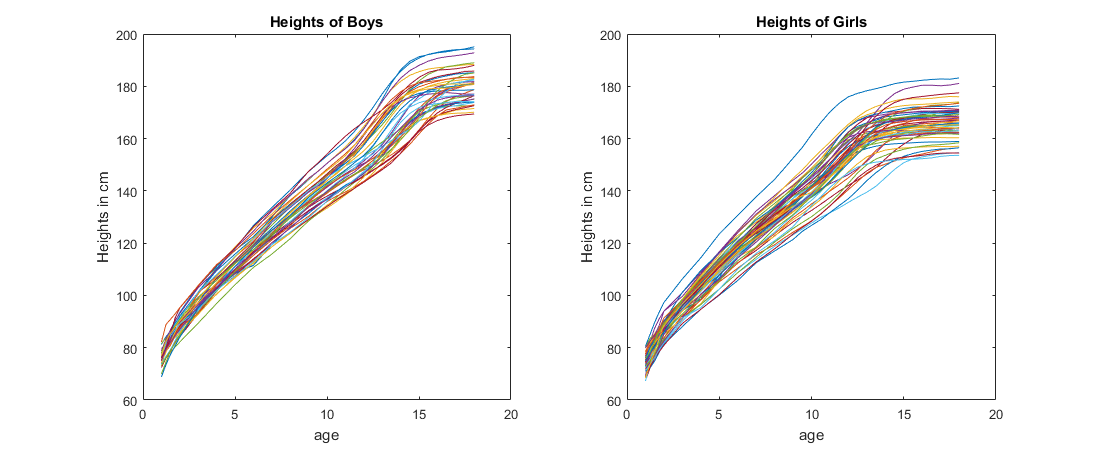
\includegraphics[scale=0.6]{hw57.png}\\
Because we are interested in the growth rates instead of absolute heights, so I first smooth the data and get a growth rate function of 2 random curves.\\
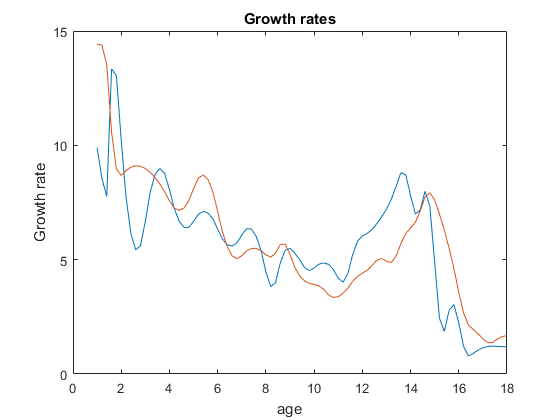
\includegraphics[scale=0.6]{hw58.png}\\
Next, I smoothed the growth rates curve and converted them to SRSF functions q1 and q2 which are ready for registration.\\
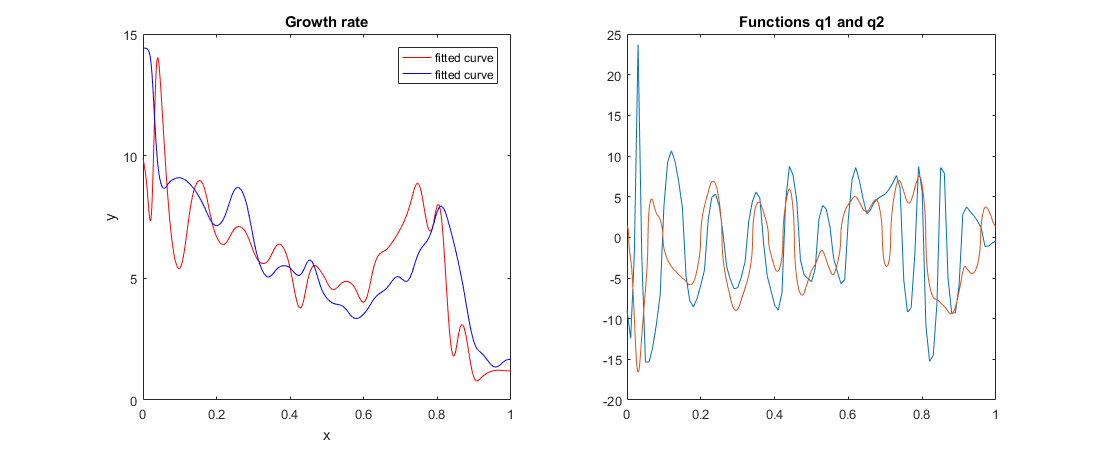
\includegraphics[scale=0.6]{hw59.png}\\
Now I applied dynamic programming with SRSF representations\\
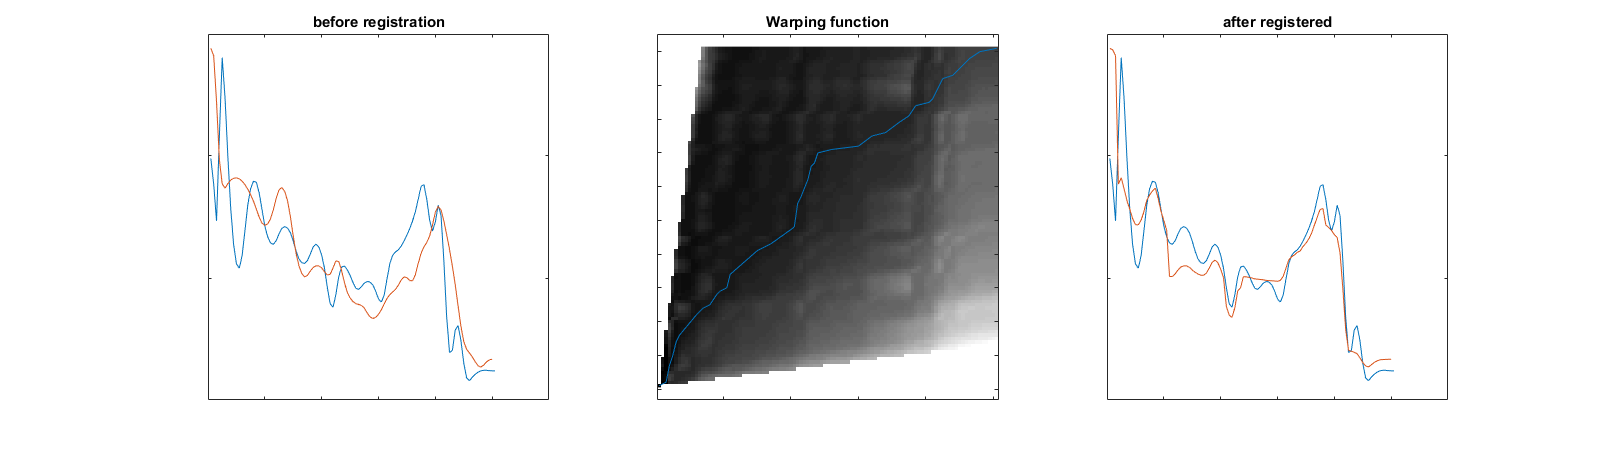
\includegraphics[scale=0.4]{hw510.png}\\
Try another pair of boys\\
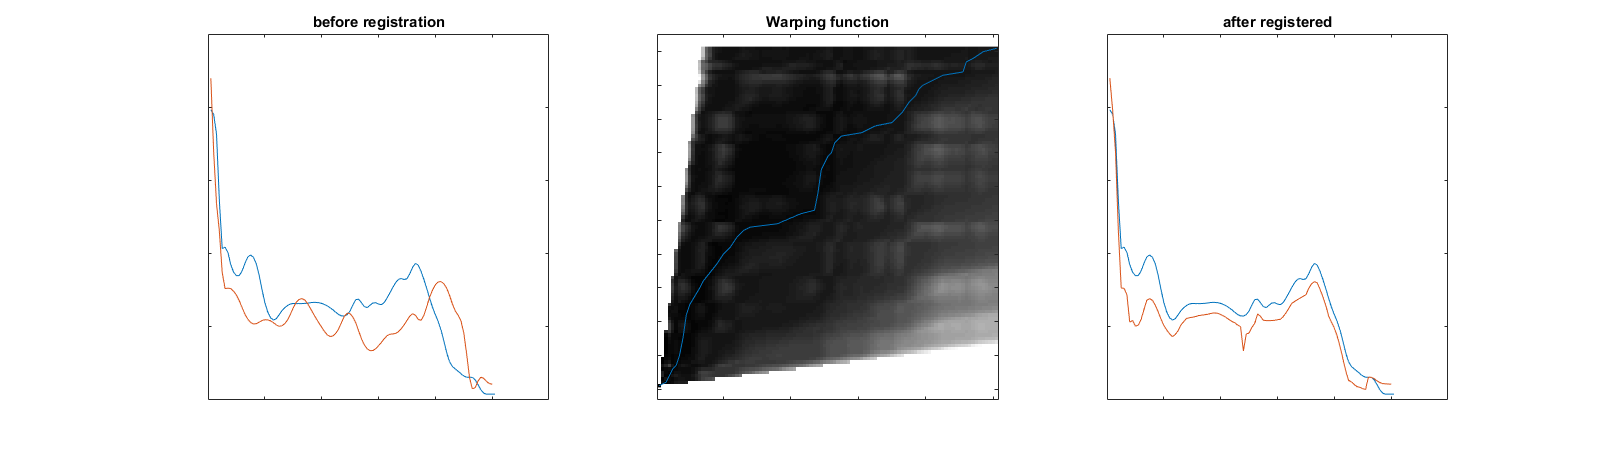
\includegraphics[scale=0.4]{hw511.png}\\
Try another pair of girls\\
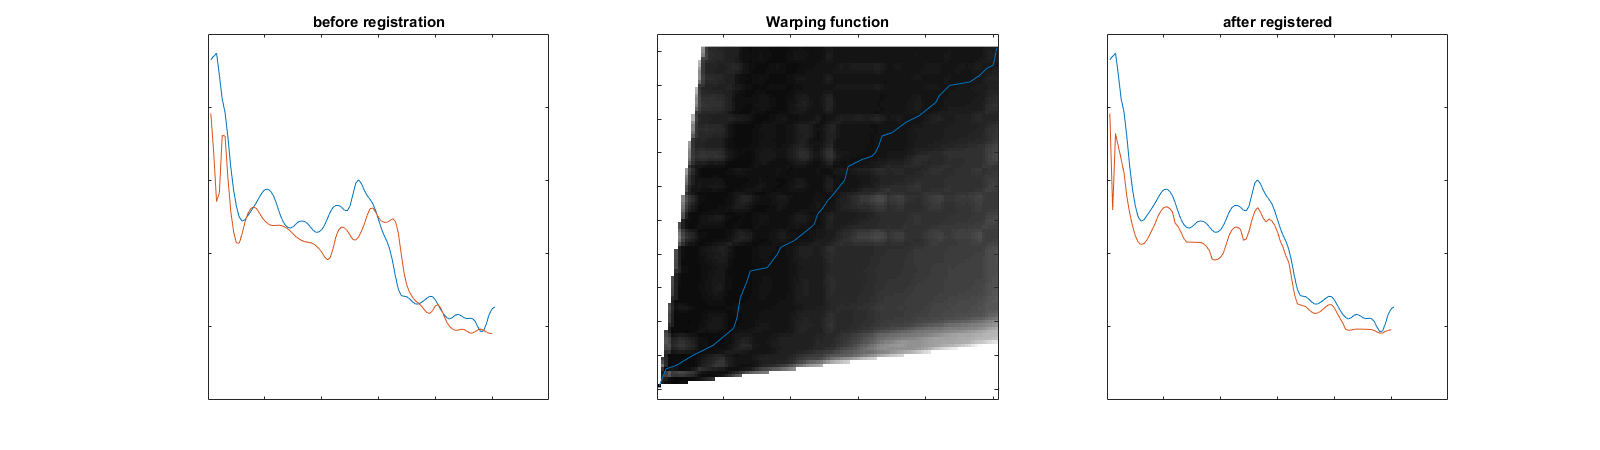
\includegraphics[scale=0.4]{hw512.png}\\
Above all, the algorithm seem to work well for growth data.

All code please see https://github.com/rikku1983/STAT5376\\
\bigskip

Thanks!


\end{document}